\chapter{Diversidade dos organismos unicelulares}\label{ch:b2:unicellular-diversity}

Uma gota de água de lagoa ao microscópio contém uma célula verde que
rema com dois flagelos, um ciliado em forma de chinelo que varre
bactérias para dentro de sua citofaringe, uma diatomácea vítrea que
desliza sobre a lâmina e, pequenas demais para serem bem vistas, mil
bactérias. Cada uma é uma só célula e cada uma é um organismo inteiro:
alimenta-se, move-se, percebe, cresce, reproduz-se e morre como uma
única célula. A maior parte do mundo vivo sempre foi assim. Este
capítulo trata o \omterm{def:b2:unicellular-diversity:unicellular}{organismo unicelular} como um problema de projeto ---
o que uma célula consegue e não consegue fazer --- e passa em revista
as respostas que os \omterm{def:b2:unicellular-diversity:prokaryote}{procariotos} e os eucariotos encontraram, até o
ponto em que as células começam a permanecer juntas.

\section{Uma célula, todas as funções}

\begin{definition}[Unicelular, colonial, multicelular]\label{def:b2:unicellular-diversity:unicellular}
Um organismo é \emph{unicelular}\index{organismo unicelular} quando
uma única célula realiza todas as funções da vida --- nutrição,
trocas, movimento, reprodução --- e vive por conta própria. É
\emph{colonial}\index{organismo colonial} quando células de um mesmo
tipo permanecem unidas depois de se dividir, mas cada uma continua
capaz de viver sozinha se for separada. É
\emph{multicelular}\index{organismo multicelular} quando suas células
são de vários tipos, dependem umas das outras e apenas algumas delas
(a linhagem germinativa) deixam descendentes. Os organismos
unicelulares incluem todas as arqueias, quase todas as bactérias e a
maioria das linhagens de eucariotos; o nome informal
\emph{\omterm{def:b2:unicellular-diversity:protist}{protista}} abrange os eucariotos unicelulares, que não formam um
grupo, mas muitos.
\end{definition}

\begin{example}[Seis habitantes de uma gota]\label{ex:b2:unicellular-diversity:drop}
\emph{Escherichia coli}, um bastonete de \qty{2}{\micro m} de
comprimento, nada com um tufo de flagelos e se divide a cada vinte
minutos quando alimentada. \emph{Chlamydomonas}, uma alga verde de
\qty{10}{\micro m} de diâmetro, rema com dois flagelos em direção à
luz que detecta com um estigma. \emph{Paramecium}, um ciliado de
\qty{200}{\micro m}, é coberto por milhares de cílios, alimenta-se por
uma citofaringe e bombeia água para fora com dois vacúolos
contráteis. Uma diatomácea vive numa carapaça de sílica em duas
partes, ornamentada de poros. A \emph{Amoeba} flui estendendo
pseudópodes e engloba o que encontra. Uma célula de levedura forma um
broto lateral, a célula-filha. Seis respostas, de tamanho e
maquinaria muito diferentes, a um mesmo problema.
\end{example}

\begin{omfigure}
\begin{tikzpicture}[x=1.9cm]
  % log scale from 0.1 um to 100 mm : position = log10(size in um) + 1
  \draw[thick] (0,0) -- (6,0);
  \foreach \p/\l in {0/{\qty{0.1}{\micro m}},1/{\qty{1}{\micro m}},2/{\qty{10}{\micro m}},3/{\qty{100}{\micro m}},4/{\qty{1}{mm}},5/{\qty{10}{mm}},6/{\qty{100}{mm}}}
    \draw (\p,0.12) -- (\p,-0.12) node[below, font=\scriptsize] {\l};
  \foreach \p/\c/\l in {0.5/omDef/micoplasma, 1.3/omDef/{\emph{E.~coli}}, 1.7/omDef/levedura, 2.0/omProp/{\emph{Chlamydomonas}}, 2.7/omProp/diatomáceas, 3.3/omProp/{\emph{Paramecium}}, 3.65/omProp/{\emph{Amoeba proteus}}, 3.9/omThm/{\emph{Thiomargarita} (uma bactéria)}, 5.7/omProp/{\emph{Acetabularia}}}
    { \fill[\c] (\p,0) circle (0.05); \node[rotate=60, anchor=west, font=\scriptsize, \c, inner sep=1pt] at (\p,0.12) {\l}; }
  \node[font=\scriptsize, anchor=north] at (3,-0.55) {tamanho celular (escala logarítmica)};
\end{tikzpicture}

{\small Os tamanhos dos \omterm{def:b2:unicellular-diversity:unicellular}{organismos unicelulares} cobrem cinco ordens de
grandeza. Os \omterm{def:b2:unicellular-diversity:prokaryote}{procariotos} (azul) concentram-se em torno de um
micrômetro; as células eucarióticas (laranja) são de dez a cem vezes
maiores; as maiores células isoladas --- uma bactéria sulfurosa
gigante, a alga \emph{Acetabularia} --- são exceções que o texto
explica.}
\end{omfigure}

\begin{proposition}[Superfície, volume e o limite de tamanho]\label{prop:b2:unicellular-diversity:surface}
\index{razão superfície/volume}
Uma célula faz trocas com o meio através de sua superfície e consome
em proporção ao seu volume. Para uma esfera de raio $r$, a
\emph{\omterm{prop:b2:unicellular-diversity:surface}{razão superfície/volume}} é
\[
\frac{S}{V} = \frac{4\pi r^2}{\tfrac{4}{3}\pi r^3} = \frac{3}{r},
\]
de modo que dobrar o raio reduz à metade a superfície disponível por
unidade de citoplasma. Uma célula que depende da difusão através da
membrana para abastecer seu interior não pode, portanto, crescer
indefinidamente: a partir de certo raio, o suprimento pela superfície
deixa de atender à demanda do volume. A mesma lei explica por que as
células pequenas são as metabolicamente mais ativas por grama, e por
que as células grandes são achatadas, alongadas, vacuoladas ou
repletas de membranas internas.
\end{proposition}

\begin{theorem}[Tempo para difundir por uma distância]\label{thm:b2:unicellular-diversity:diffusion}
\index{tempo de difusão}
Uma molécula de coeficiente de difusão $D$ vagueia em passos
aleatórios; após um tempo $t$, seu deslocamento quadrático médio ao
longo de um eixo é $\langle x^2\rangle = 2Dt$. O tempo necessário para
percorrer uma distância $x$ apenas por difusão é, portanto,
\[
t \approx \frac{x^2}{2D},
\]
que cresce com o \emph{quadrado} da distância. Com
$D \approx \qty{1e-9}{m^2/s}$ para uma molécula pequena na água,
atravessar uma bactéria (\qty{1}{\micro m}) leva meio milissegundo;
atravessar uma célula de \qty{1}{mm} levaria oito minutos, e um metro,
dezesseis anos.
\end{theorem}
\begin{proof}
Suponha que a molécula dê passos de comprimento $\ell$ ao acaso para a
esquerda ou para a direita a cada $\tau$ segundos. Após $n$ passos, seu
deslocamento é $x = \sum_i \varepsilon_i \ell$ com
$\varepsilon_i = \pm 1$ independentes, de modo que
$\langle x\rangle = 0$ e $\langle x^2\rangle =
\sum_i \langle\varepsilon_i^2\rangle \ell^2 = n\ell^2$ (os termos
cruzados têm média nula). Com $n = t/\tau$, isso dá $\langle x^2\rangle
= (\ell^2/\tau)\,t$, e escrevendo $D = \ell^2/2\tau$ obtém-se
$\langle x^2\rangle = 2Dt$. Fazendo $\langle x^2\rangle = x^2$, obtém-se
o tempo.
\end{proof}

\begin{theorem}[Suprimento por difusão a uma célula esférica]\label{thm:b2:unicellular-diversity:supply}
\index{absorção limitada pela difusão}
Uma célula esférica de raio $r_0$ que absorve toda molécula de um
soluto que alcança sua superfície, num meio em que a concentração ao
longe é $c_\infty$, recebe em regime estacionário um fluxo (moléculas
por segundo) de
\[
J = 4\pi D r_0\, c_\infty .
\]
O suprimento cresce apenas com $r_0$, enquanto a demanda cresce com
$r_0^3$: além de certo raio, uma célula alimentada por difusão passa
fome.
\end{theorem}
\begin{proof}
Em regime estacionário, o número de moléculas que atravessam por
segundo cada esfera de raio $r > r_0$ é o mesmo, $J = 4\pi r^2 D\,
(\mathrm{d}c/\mathrm{d}r)$ (lei de Fick, com o fluxo dirigido para
dentro). Assim, $r^2\,\mathrm{d}c/\mathrm{d}r = J/4\pi D$ é constante;
integrando de $r_0$, onde $c = 0$, até o infinito, onde
$c = c_\infty$:
$c_\infty = (J/4\pi D)\int_{r_0}^{\infty} r^{-2}\,\mathrm{d}r =
J/(4\pi D r_0)$, donde $J = 4\pi D r_0 c_\infty$.
\end{proof}

\begin{example}[Qual o tamanho máximo de uma célula alimentada por difusão?]\label{ex:b2:unicellular-diversity:howbig}
Uma célula aeróbia consome oxigênio a cerca de
$q = \qty{0.02}{mol/m^3/s}$ de citoplasma (um ritmo intenso). Sua
demanda é $q \cdot \tfrac{4}{3}\pi
r_0^3$; o suprimento a partir de água saturada de ar ($c_\infty =
\qty{0.25}{mol/m^3}$, $D = \qty{2e-9}{m^2/s}$) é $4\pi D r_0
c_\infty$. Igualando, $r_0^2 = 3Dc_\infty/q = 3\times 2\times 10^{-9}
\times 0.25/0.02 = \qty{7.5e-8}{m^2}$, de modo que $r_0 \approx
\qty{270}{\micro m}$. As células ativas reais ficam bem abaixo disso,
porque o oxigênio também precisa se difundir \emph{dentro} delas; a
bactéria sulfurosa \emph{Thiomargarita}, de \qty{750}{\micro m},
contorna o limite sendo quase inteiramente um vacúolo, com o
citoplasma reduzido a uma casca fina de alguns micrômetros de
espessura.
\end{example}

\begin{omfigure}
\begin{tikzpicture}
\begin{axis}[
  width=0.8\linewidth, height=6.2cm,
  axis x line=bottom, axis y line=left,
  xmode=log, ymode=log,
  xmin=0.3, xmax=1000, ymin=1e-6, ymax=1e4,
  xlabel={raio celular (\unit{\micro m})}, ylabel={moléculas por segundo (relativo)},
  xlabel style={font=\small, at={(axis description cs:0.5,-0.1)}, anchor=north},
  ylabel style={font=\small},
  tick label style={font=\small},
  legend style={font=\small, at={(0.03,0.97)}, anchor=north west, draw=none},
  clip=false,
]
\addplot[very thick, omDef, domain=0.3:1000, samples=40] {x/10};
\addlegendentry{suprimento por difusão, $\propto r$}
\addplot[very thick, omThm, domain=0.3:1000, samples=40] {(x/10)^3/1000*1.0};
\addlegendentry{demanda do citoplasma, $\propto r^3$}
\draw[dashed, gray] (axis cs:270,1e-6) -- (axis cs:270,27);
\node[font=\scriptsize, anchor=west] at (axis cs:300,3e-4) {raio de inanição};
\end{axis}
\end{tikzpicture}

{\small O suprimento pela superfície cresce com $r$, a demanda com
$r^3$ (eixos logarítmicos). Onde as retas se cruzam, uma célula
alimentada apenas por difusão já não consegue abastecer seu interior;
o cruzamento fica perto de algumas centenas de micrômetros para uma
célula aeróbia ativa.}
\end{omfigure}

\section{Diversidade procariótica}

\begin{definition}[A célula procariótica]\label{def:b2:unicellular-diversity:prokaryote}
Um \emph{procarioto}\index{procarioto} (as bactérias e as arqueias,
dois domínios tão distintos entre si quanto cada um deles o é de nós) é
uma célula sem núcleo nem organelas delimitadas por membrana: um único
cromossomo circular num \emph{nucleoide}\index{nucleoide}, muitas vezes
acompanhado de pequenos círculos adicionais chamados
\emph{plasmídeos}\index{plasmídeo}, ribossomos livres num citoplasma
de \qtyrange{0.5}{2}{\micro m}, uma membrana plasmática que abriga as
cadeias respiratórias ou fotossintéticas, e uma
\emph{parede celular}\index{parede celular!bacteriana} rígida que
resiste à turgescência de um citoplasma vários bares acima do meio
externo. As formas são poucas e têm nome: \emph{coco} (esfera),
\emph{bacilo} (bastonete), \emph{espirilo} e \emph{espiroqueta}
(hélices), \emph{vibrião} (vírgula); as células podem permanecer aos
pares, em cadeias, em tétrades ou em cachos depois de se dividir.
\end{definition}

\begin{proposition}[Dois envoltórios: Gram-positivo e Gram-negativo]\label{prop:b2:unicellular-diversity:gram}
\index{coloração de Gram}\index{peptidoglicano}
A parede bacteriana é feita de \emph{peptidoglicano}, cadeias de dois
açúcares alternados unidas por peptídeos curtos numa única molécula
gigante em torno da célula. As bactérias \emph{Gram-positivas} têm
uma camada espessa (\qtyrange{20}{80}{nm}) por fora de uma única
membrana e retêm o cristal violeta da \omterm{prop:b2:unicellular-diversity:gram}{coloração de Gram}; as bactérias
\emph{Gram-negativas} têm uma camada fina (alguns nanômetros) entre a
membrana plasmática e uma \emph{membrana externa} cujo folheto externo
é feito de lipopolissacarídeo, e perdem o corante. A membrana
externa, perfurada por porinas, é uma segunda barreira: barra muitos
antibióticos e detergentes, e é por isso que as infecções por
Gram-negativos são mais difíceis de tratar. As arqueias não têm nem
peptidoglicano nem os lipídios ligados por éster de todas as outras
células: suas membranas são feitas de cadeias isoprenoides ligadas
por éter, que às vezes atravessam toda a bicamada como uma monocamada,
o que as mantém estáveis em ácido fervente.
\end{proposition}

\begin{omfigure}
\begin{tikzpicture}[scale=0.9, every node/.style={font=\scriptsize}]
  % Gram-positive
  \begin{scope}
    \fill[omDef!15] (0,0) rectangle (4,1.6);
    \node at (2,0.4) {citoplasma};
    \fill[omDef!60] (0,1.6) rectangle (4,1.85);
    \node[right] at (4.05,1.72) {membrana plasmática};
    \fill[omProp!50] (0,1.85) rectangle (4,3.0);
    \foreach \y in {2.0,2.25,...,2.85} \draw[omProp!90!black] (0.1,\y) -- (3.9,\y);
    \node[right, align=left] at (4.05,2.45) {peptidoglicano espesso\\(\qtyrange{20}{80}{nm})};
    \node[above, font=\small\bfseries] at (2,3.05) {Gram-positiva};
  \end{scope}
  % Gram-negative
  \begin{scope}[xshift=7.6cm]
    \fill[omDef!15] (0,0) rectangle (4,1.6);
    \node at (2,0.4) {citoplasma};
    \fill[omDef!60] (0,1.6) rectangle (4,1.85);
    \node[right] at (4.05,1.72) {membrana plasmática};
    \fill[omProp!50] (0,2.05) rectangle (4,2.25);
    \draw[omProp!90!black] (0.1,2.15) -- (3.9,2.15);
    \node[right] at (4.05,2.15) {peptidoglicano fino};
    \node at (2,1.95) {periplasma};
    \fill[omThm!50] (0,2.55) rectangle (4,2.85);
    \foreach \x in {0.6,2.0,3.4} \fill[white] (\x-0.12,2.55) rectangle (\x+0.12,2.85);
    \node[right] at (4.05,2.7) {membrana externa com porinas};
    \foreach \x in {0.2,0.5,...,3.9} \draw[omThm!80!black, thick] (\x,2.85) -- (\x,3.1);
    \node[right] at (4.05,3.15) {lipopolissacarídeo};
    \node[above, font=\small\bfseries] at (2,3.3) {Gram-negativa};
  \end{scope}
\end{tikzpicture}

{\small Os dois envoltórios bacterianos em corte. À esquerda: uma
membrana sob uma espessa camada de peptidoglicano. À direita: uma
camada fina de peptidoglicano no periplasma, entre duas membranas, a
externa cravejada de porinas e revestida de lipopolissacarídeo.}
\end{omfigure}

\begin{proposition}[O flagelo bacteriano e a quimiotaxia]\label{prop:b2:unicellular-diversity:flagellum}
\index{flagelo!bacteriano}\index{quimiotaxia}
O \emph{flagelo} bacteriano é um filamento helicoidal rígido da
proteína flagelina, com \qty{20}{nm} de espessura e várias vezes o
comprimento do corpo, girado por um motor rotativo inserido no
envoltório. O motor não é movido por ATP, mas por prótons que descem
o gradiente eletroquímico através da membrana, à razão de cerca de
\num{1000} prótons por volta e até \num{300} voltas por segundo. Em
\emph{E.~coli}, os vários flagelos se juntam num feixe quando todos
giram no sentido anti-horário e empurram a célula numa
\emph{corrida} em linha reta; quando um ou mais se invertem, o feixe se
desfaz e a célula \emph{cambalhota}, tomando uma nova direção
aleatória. A \emph{quimiotaxia} é o viés desse passeio aleatório: a
célula mede se a concentração de um atraente aumentou durante o
último segundo e, se for o caso, suprime as cambalhotas. Ela se
orienta comparando o presente com o passado recente --- ao longo de
sua trajetória --- porque, ao longo de seu próprio
\qty{1}{\micro m} de comprimento, nenhum gradiente é mensurável.
\end{proposition}
\begin{proof}[Evidências]
Berg e Brown (1972) seguiram células isoladas de \emph{E.~coli} em
três dimensões com um microscópio de rastreamento: corridas de cerca
de um segundo a \qty{20}{\micro m/s}, cambalhotas de um décimo de
segundo e, num gradiente de serina, corridas mais longas no sentido
ascendente do gradiente, sem que as corridas no sentido descendente
fossem encurtadas. Prender uma célula a uma lâmina de vidro por um
único flagelo fazia o corpo inteiro girar, o que provou que o motor é
rotativo; células com o motor desacoplado da síntese de ATP
continuavam a nadar enquanto se pudesse impor um gradiente de
prótons, o que identificou o combustível.
\end{proof}

\begin{omfigure}
\begin{tikzpicture}[every node/.style={font=\scriptsize}]
  % run and tumble path without gradient
  \begin{scope}
    \draw[very thick, omDef] (0,0) -- (1.2,0.5) -- (0.7,1.4) -- (1.9,1.8) -- (2.6,0.9) -- (3.4,1.5) -- (3.0,2.5);
    \foreach \p in {(1.2,0.5),(0.7,1.4),(1.9,1.8),(2.6,0.9),(3.4,1.5)} \fill[omThm] \p circle (0.06);
    \node[align=center] at (1.8,-0.5) {sem gradiente:\\corridas de igual comprimento, giros aleatórios};
  \end{scope}
  \begin{scope}[xshift=6cm]
    \shade[left color=white, right color=omExo!50] (-0.3,-0.2) rectangle (5.2,3.0);
    \draw[very thick, omDef] (0,0.3) -- (0.9,0.8) -- (0.6,1.3) -- (2.4,1.5) -- (2.2,2.2) -- (4.6,2.4);
    \foreach \p in {(0.9,0.8),(0.6,1.3),(2.4,1.5),(2.2,2.2)} \fill[omThm] \p circle (0.06);
    \node[align=center] at (2.4,-0.5) {atraente crescendo para a direita:\\as corridas gradiente acima duram mais};
    \node[anchor=south east] at (5.1,2.6) {mais atraente};
  \end{scope}
\end{tikzpicture}

{\small Corrida e cambalhota. À esquerda: sem gradiente, a célula
executa um passeio aleatório, cada corrida (azul) terminada por uma
cambalhota (ponto vermelho). À direita: quando um atraente aumenta ao
longo de uma corrida, a cambalhota é suprimida e a corrida se alonga;
o passeio deriva gradiente acima.}
\end{omfigure}

\begin{example}[As cianobactérias e o heterocisto]\label{ex:b2:unicellular-diversity:cyanobacteria}
As cianobactérias são as bactérias que fazem fotossíntese como as
plantas, quebrando a água e liberando oxigênio em membranas internas
empilhadas (os tilacoides, que o cloroplasto herdou delas). Muitas
crescem como filamentos de células que compartilham uma bainha. Em
\emph{Anabaena}, quando o nitrogênio combinado se esgota, cerca de uma
célula em cada dez se torna um \emph{heterocisto}: desmonta seu
fotossistema produtor de oxigênio, espessa a parede contra o oxigênio
e fixa o nitrogênio atmosférico com uma enzima que o oxigênio
destruiria, exportando glutamina para as vizinhas em troca de açúcar.
Um filamento de \emph{Anabaena} é um primeiro esboço de divisão de
trabalho entre células.
\end{example}

\begin{omfigure}
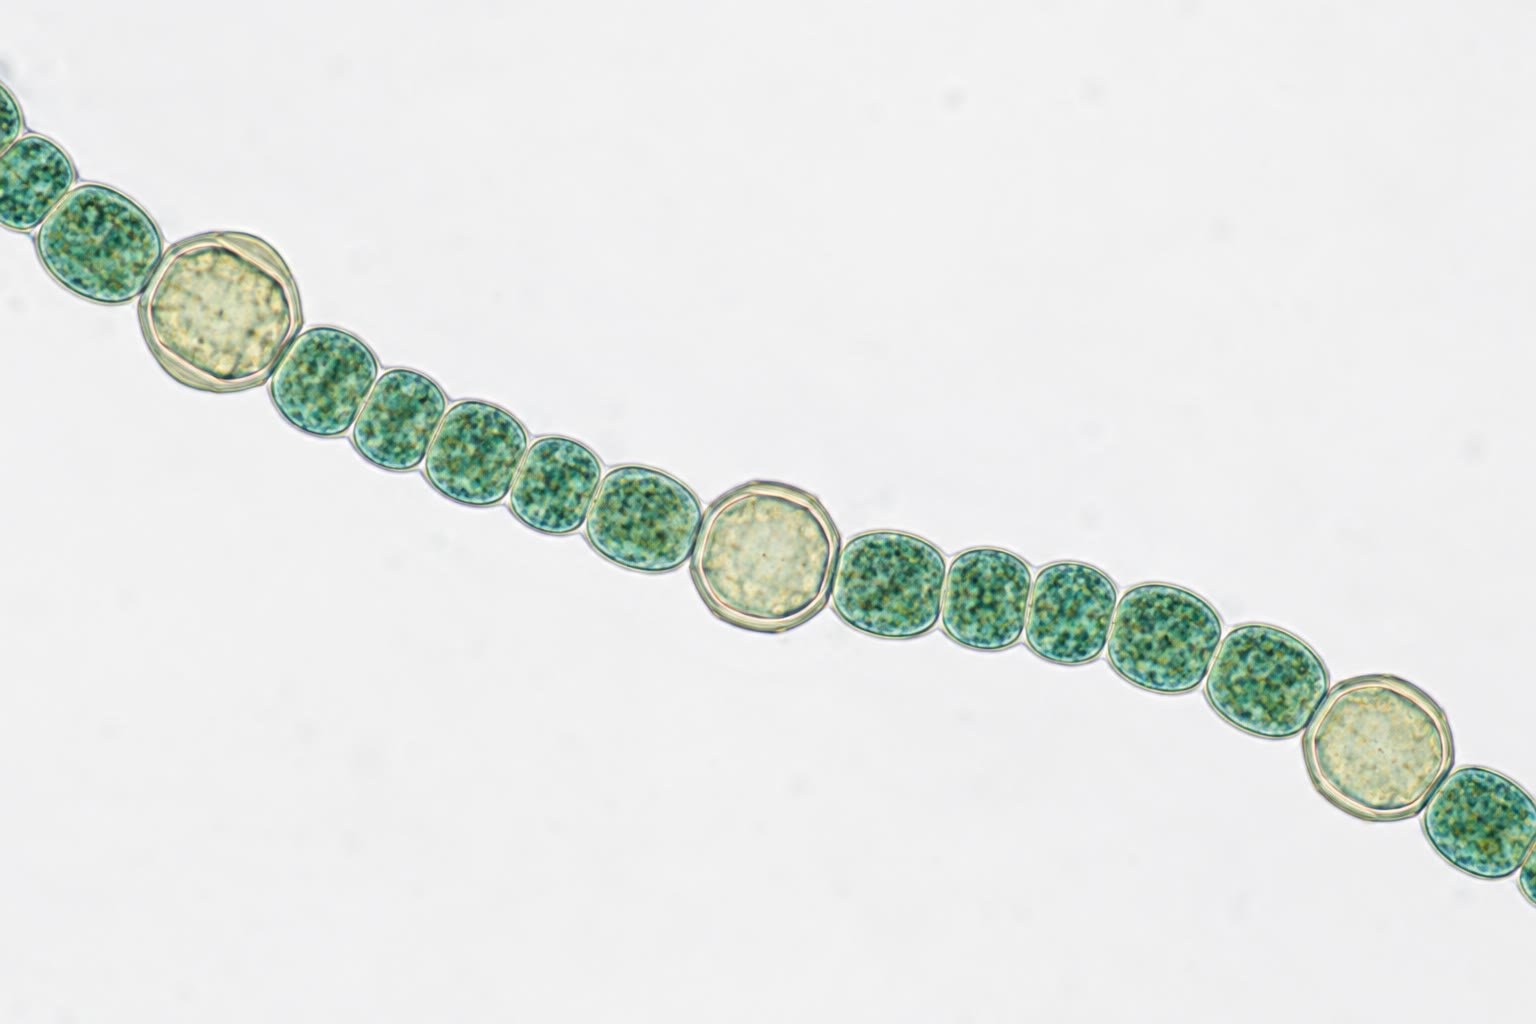
\includegraphics[width=0.62\linewidth]{images/book4/ai/b4-01-anabaena.jpg}

{\small Um filamento de \emph{Anabaena}: uma cadeia de células
fotossintéticas verdes interrompida por heterocistos maiores e mais
pálidos, as células que fixam nitrogênio.}
\end{omfigure}

\begin{remark}[Dormência]\label{rem:b2:unicellular-diversity:spores}
Alguns bastonetes Gram-positivos (\emph{Bacillus}, \emph{Clostridium})
respondem à escassez de alimento construindo um \emph{endósporo}: uma
cópia do cromossomo envolta em vários revestimentos desidratados,
metabolicamente inerte, resistente à fervura, à radiação e a séculos
de seca, que germina quando as condições voltam. Muitos \omterm{def:b2:unicellular-diversity:protist}{protistas}
fazem o mesmo com um \emph{cisto}. A dormência é a outra maneira de
sobreviver a uma estação ruim, ao lado da motilidade.
\end{remark}

\section{Os eucariotos unicelulares}

\begin{definition}[Protistas: um grau, não um grupo]\label{def:b2:unicellular-diversity:protist}
Os \emph{protistas}\index{protista} são os eucariotos que não são nem
animais, nem plantas terrestres, nem fungos --- em sua maioria
\omterm{def:b2:unicellular-diversity:unicellular}{unicelulares}, alguns \omterm{def:b2:unicellular-diversity:unicellular}{coloniais}, uns poucos (as laminárias)
\omterm{def:b2:unicellular-diversity:unicellular}{multicelulares}. Compartilham a célula eucariótica do volume do Ano 1
(núcleo, mitocôndrias, endomembranas, citoesqueleto, cílios $9+2$) e
nada mais em particular: as linhagens que os contêm são tão distantes
umas das outras quanto os animais o são das plantas. As algas verdes
pertencem ao ramo das plantas terrestres; as diatomáceas e as algas
pardas formam uma linhagem própria; os ciliados, os dinoflagelados e
o parasita da malária formam outra; as amebas e os mixomicetos estão
mais próximos dos animais e dos fungos do que de qualquer um desses.
A palavra designa um nível de organização --- a célula eucariótica
vivendo sozinha --- e não um ramo da árvore.
\end{definition}

\begin{example}[Quatro maneiras de ser uma célula eucariótica sozinha]\label{ex:b2:unicellular-diversity:four}
\emph{Chlamydomonas}: uma alga verde ovoide com uma parede de
glicoproteína sem celulose, um cloroplasto em forma de taça, um
estigma alaranjado que sombreia um sensor de luz, de modo que a célula
sabe de que lado vem a luz enquanto gira, e dois flagelos anteriores
que batem como num nado de peito; é fototrófica.
\emph{Paramecium}: um ciliado, com toda a superfície batendo cílios em
ondas coordenadas, um sulco oral semelhante a uma boca que varre
bactérias para vacúolos digestivos, dois vacúolos contráteis e dois
tipos de núcleo --- um pequeno \emph{micronúcleo} germinativo e um
grande \emph{macronúcleo} funcional, com centenas de cópias de cada
gene; é fagotrófico. \emph{Amoeba}: sem parede, sem forma fixa, move-se
e se alimenta por \emph{pseudópodes} projetados pela polimerização da
actina. A diatomácea: uma célula fotossintética encerrada em duas
valvas de sílica sobrepostas como uma caixa e sua tampa, tão
ornamentadas de poros que as carapaças já serviram para testar
lentes de microscópio; quando ela se divide, cada filha conserva uma
valva e fabrica uma nova valva interna, menor.
\end{example}

\begin{omfigure}
\begin{tikzpicture}[every node/.style={font=\scriptsize}]
  % Paramecium outline (slipper)
  \draw[thick, fill=omProp!8] plot[smooth cycle, tension=0.8] coordinates {(0,0) (1.5,0.9) (3.5,1.1) (5.5,0.7) (6.4,0) (5.5,-0.8) (3.5,-1.1) (1.5,-0.9)};
  % cilia
  \foreach \t in {3,9,...,357} {
    \pgfmathsetmacro{\cx}{3.2+3.25*cos(\t)}
    \pgfmathsetmacro{\cy}{1.08*sin(\t)}
    \pgfmathsetmacro{\dx}{3.2+3.55*cos(\t)}
    \pgfmathsetmacro{\dy}{1.32*sin(\t)}
    \draw[gray] (\cx,\cy) -- (\dx,\dy);
  }
  % macronucleus and micronucleus
  \draw[thick, fill=omDef!40] (3.2,0.05) ellipse (0.9 and 0.45);
  \fill[omDef!90!black] (2.4,0.55) circle (0.13);
  % oral groove and gullet
  \draw[thick, omThm] (4.3,-0.95) .. controls (3.6,-0.5) and (3.3,-0.2) .. (3.0,-0.35);
  \fill[omThm!30] (2.9,-0.45) circle (0.16);
  % food vacuoles
  \foreach \p in {(1.4,-0.3),(1.0,0.35),(4.8,0.35)} \draw[thick, omExo!80!black, fill=omExo!30] \p circle (0.17);
  % contractile vacuoles
  \foreach \c in {(1.2,0.0),(5.2,-0.2)} {
    \draw[thick, omDef] \c circle (0.28);
    \foreach \a in {0,60,...,300} \draw[omDef] \c ++(\a:0.28) -- ++(\a:0.22);
  }
  % labels
  \draw (2.4,0.55) -- (2.7,1.6) node[above] {micronúcleo};
  \draw (3.6,0.3) -- (4.8,1.6) node[above] {macronúcleo};
  \draw (1.2,0.28) -- (0.3,1.5) node[above, align=center] {vacúolo contrátil\\(com canais radiais)};
  \draw (5.2,-0.48) -- (6.5,-1.5) node[below] {vacúolo contrátil};
  \draw (4.3,-0.95) -- (4.7,-1.75) node[below] {sulco oral};
  \draw (2.9,-0.61) -- (2.7,-1.6) node[below, align=center] {citofaringe e vacúolo\\digestivo em formação};
  \draw (1.4,-0.47) -- (0.0,-1.5) node[below] {vacúolos digestivos};
  \draw (6.35,0.4) -- (6.9,1.2) node[above, align=center] {cílios};
\end{tikzpicture}

{\small \emph{Paramecium}, esquema: o córtex ciliado, os dois núcleos,
o sulco oral que leva à citofaringe, onde se formam os vacúolos
digestivos, e os dois vacúolos contráteis em forma de estrela que
expulsam a água que a osmose faz entrar.}
\end{omfigure}

\begin{omfigure}
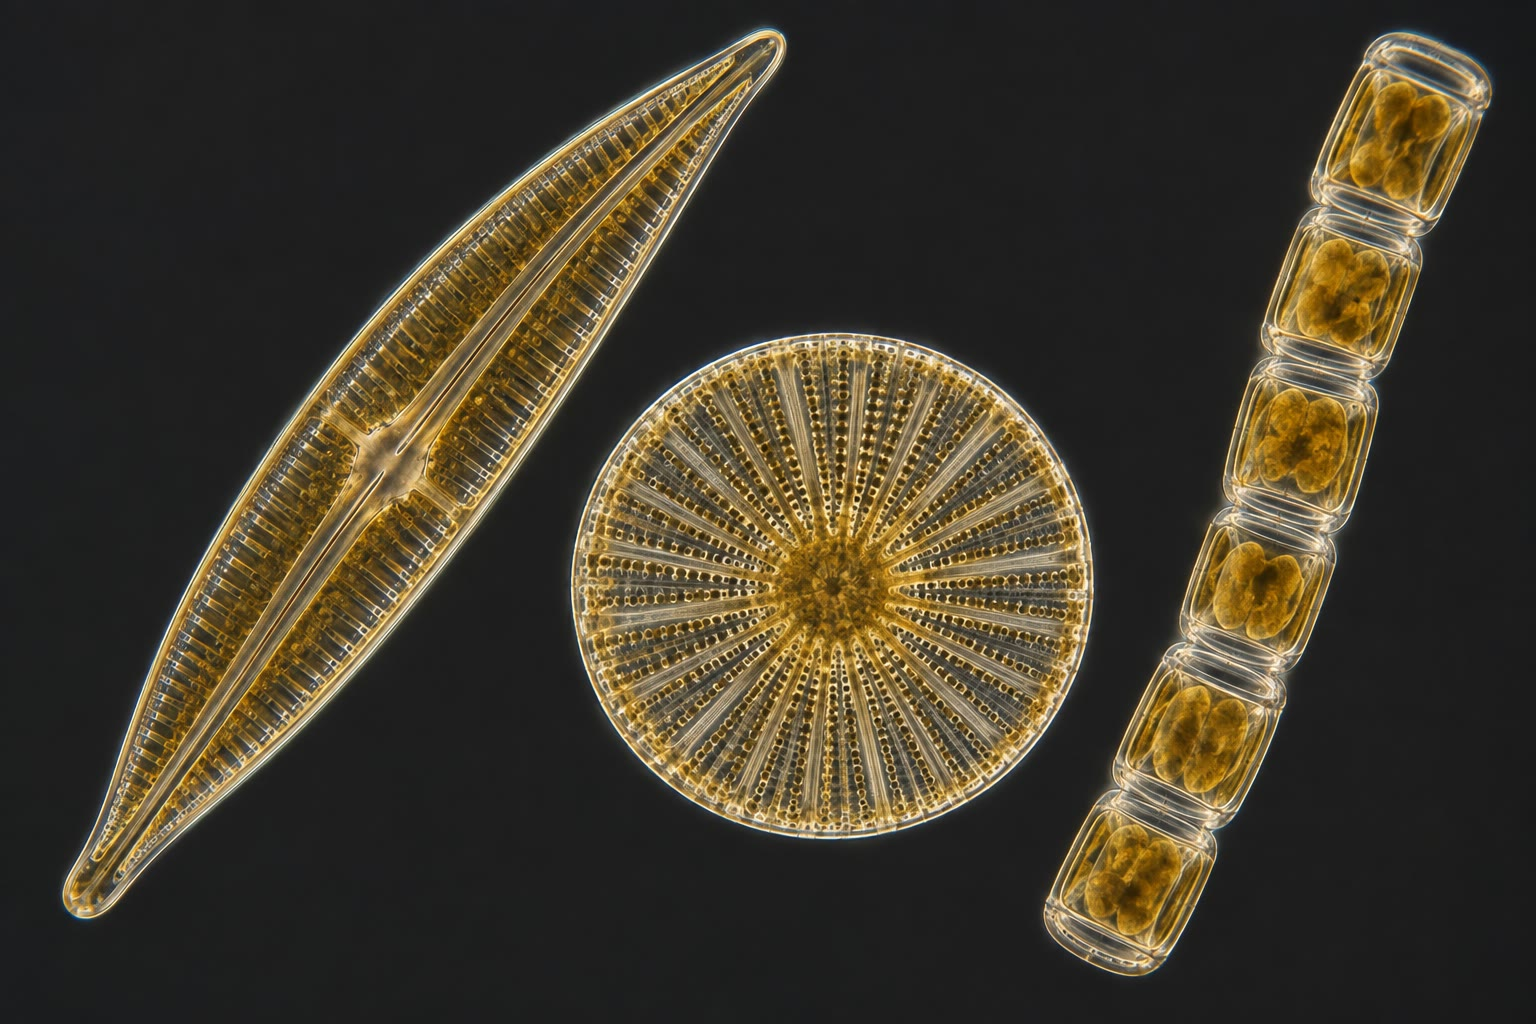
\includegraphics[width=0.6\linewidth]{images/book4/ai/b4-01-diatoms.jpg}

{\small Diatomáceas vistas em microscopia de campo escuro: cada célula
vive numa carapaça de sílica de duas valvas, marcada por poros através
dos quais faz trocas com a água.}
\end{omfigure}

\begin{definition}[Modos de nutrição]\label{def:b2:unicellular-diversity:nutrition}
\index{fagotrofia}\index{osmotrofia}\index{mixotrofia}
Um eucarioto \omterm{def:b2:unicellular-diversity:unicellular}{unicelular} alimenta-se de uma de três maneiras, ou de
duas ao mesmo tempo. \emph{Fototrofia}: tem cloroplastos e produz sua
própria matéria orgânica a partir da luz e do $\mathrm{CO_2}$ (algas
verdes, diatomáceas, dinoflagelados). \emph{Fagotrofia}: engloba
partículas --- bactérias, outros \omterm{def:b2:unicellular-diversity:protist}{protistas} --- num vacúolo digestivo
onde enzimas lisossômicas as digerem (amebas, ciliados,
coanoflagelados). \emph{Osmotrofia}: absorve moléculas dissolvidas
através da membrana, muitas vezes depois de secretar enzimas para
fora (leveduras, muitos parasitas). Os \emph{mixotróficos}, como a
\emph{Euglena}, fazem fotossíntese na luz e comem no escuro. Os
\omterm{def:b2:unicellular-diversity:prokaryote}{procariotos} não conseguem fagocitar: a parede os impede, e é por isso
que nenhum \omterm{def:b2:unicellular-diversity:prokaryote}{procarioto} se tornou predador por englobamento.
\end{definition}

\begin{proposition}[Osmorregulação em água doce]\label{prop:b2:unicellular-diversity:osmoregulation}
\index{vacúolo contrátil}
Um \omterm{def:b2:unicellular-diversity:protist}{protista} de água doce é muito mais salgado por dentro (cerca de
\qty{100}{mmol/L} de solutos) do que a lagoa (cerca de
\qty{1}{mmol/L}), e sua membrana deixa passar a água. A água entra,
portanto, continuamente por osmose, a uma taxa proporcional à área da
superfície e à diferença de pressão osmótica
$\Delta\Pi = RT\,\Delta c$ --- cerca de \qty{2.4}{bar} para os valores
acima. Uma célula com parede resiste pela turgescência; uma célula nua
incharia e estouraria em minutos. O \emph{\omterm{prop:b2:unicellular-diversity:osmoregulation}{vacúolo contrátil}} é a
resposta: um reservatório alimentado por canais radiais, que se enche
de água bombeada por transportadores movidos por prótons e depois se
contrai, expulsando a água por um poro, a cada poucos segundos ou a
cada poucos minutos. Um \emph{Paramecium} expele o próprio volume em
água a cada meia hora; seus parentes marinhos, num meio tão salgado
quanto eles mesmos, não têm \omterm{prop:b2:unicellular-diversity:osmoregulation}{vacúolo contrátil} algum.
\end{proposition}

\section{A física de um pequeno nadador}

\begin{proposition}[A vida em baixo número de Reynolds]\label{prop:b2:unicellular-diversity:reynolds}
\index{número de Reynolds}
O \emph{\omterm{prop:b2:unicellular-diversity:reynolds}{número de Reynolds}} $Re = \rho v L/\eta$ compara as forças
inerciais às forças viscosas para um corpo de tamanho $L$ que se move
à velocidade $v$ num fluido de densidade $\rho$ e viscosidade $\eta$.
Para um nadador humano, vale cerca de $10^6$; para o
\emph{Paramecium} (\qty{200}{\micro m}, \qty{1}{mm/s}), vale 0.2, e
para uma bactéria, $10^{-5}$. Abaixo de
$Re \approx 1$ a inércia é irrelevante: uma célula que para de bater
os flagelos para de se mover em menos de um nanômetro, a água parece
um xarope espesso, e um movimento recíproco (o mesmo golpe para a
frente e para trás) não produz deslocamento algum. Os pequenos
nadadores usam, portanto, golpes não recíprocos: a hélice giratória
do flagelo bacteriano, o batimento assimétrico de um cílio (golpe
efetivo rígido, golpe de recuperação curvado), o nado de peito da
\emph{Chlamydomonas}.
\end{proposition}

\begin{theorem}[Lei de Stokes e sedimentação]\label{thm:b2:unicellular-diversity:stokes}
\index{lei de Stokes}
Uma esfera de raio $r$ e densidade $\rho_{\text{célula}}$ que se move
lentamente num fluido de viscosidade $\eta$ sofre um arrasto
$F = 6\pi\eta r v$. Deixada livre na água de densidade $\rho$, ela
afunda à velocidade terminal
\[
v_s = \frac{2\,r^2\,(\rho_{\text{célula}} - \rho)\,g}{9\eta},
\]
proporcional ao quadrado de seu raio: uma célula dez vezes maior
afunda cem vezes mais depressa. É por isso que o fitoplâncton é
pequeno, que as diatomáceas têm espinhos e gotículas de óleo, e que uma
\emph{Chlamydomonas} que para de nadar afunda para fora da luz em
poucos dias.
\end{theorem}
\begin{proof}
Na velocidade terminal, o arrasto equilibra o peso aparente (peso
menos empuxo): $6\pi\eta r v_s = \tfrac{4}{3}\pi r^3
(\rho_{\text{célula}} - \rho) g$. Isolando $v_s$, obtém-se a fórmula.
A própria lei do arrasto é deduzida na série de física para
$Re \ll 1$; aqui ela é admitida.
\end{proof}

\begin{example}[A queda de uma diatomácea]\label{ex:b2:unicellular-diversity:fall}
Uma diatomácea cêntrica de raio \qty{10}{\micro m}, \qty{100}{kg/m^3}
mais densa que a água do mar ($\eta = \qty{1e-3}{Pa.s}$), afunda a
$v_s = 2\times 10^{-10}\times 100\times 9.81/(9\times 10^{-3}) =
\qty{2.2e-5}{m/s}$, cerca de \qty{2}{m} por dia: sairia da camada
iluminada de \qty{50}{m} em menos de um mês. Suas populações
sobrevivem porque a turbulência agita a água, porque gotículas de óleo
e uma densidade baixa reduzem $\rho_{\text{célula}} - \rho$, e porque
uma célula que afunda e se divide no caminho deixa descendentes que
voltam a ser erguidos.
\end{example}

\begin{omfigure}
\begin{tikzpicture}
\begin{axis}[
  width=0.8\linewidth, height=6.0cm,
  axis x line=bottom, axis y line=left,
  xmode=log, ymode=log,
  xmin=0.5, xmax=200, ymin=1e-3, ymax=1e4,
  xlabel={raio (\unit{\micro m})}, ylabel={velocidade de sedimentação (\unit{\micro m/s})},
  xlabel style={font=\small, at={(axis description cs:0.5,-0.1)}, anchor=north},
  ylabel style={font=\small},
  tick label style={font=\small},
  clip=false,
]
\addplot[very thick, omDef, domain=0.5:200, samples=40] {0.218*x^2};
\addplot[only marks, mark=*, mark size=1.8pt, omThm] coordinates {(1,0.218) (10,21.8) (100,2180)};
\node[font=\scriptsize, anchor=west] at (axis cs:1.15,0.218) {bactéria};
\node[font=\scriptsize, anchor=west] at (axis cs:11.5,21.8) {diatomácea};
\node[font=\scriptsize, anchor=east] at (axis cs:85,2180) {protista grande};
\end{axis}
\end{tikzpicture}

{\small Velocidade de sedimentação de Stokes em função do raio para
células \qty{100}{kg/m^3} mais densas que a água. A inclinação 2 em
eixos logarítmicos é a lei em $r^2$: uma bactéria afunda um centímetro
por dia, um \omterm{def:b2:unicellular-diversity:protist}{protista} grande uns dois metros por hora.}
\end{omfigure}

\section{Reprodução e sexo numa só célula}

\begin{definition}[Modos de divisão]\label{def:b2:unicellular-diversity:division}
\index{fissão binária}\index{brotamento}\index{fissão múltipla}
Um \omterm{def:b2:unicellular-diversity:unicellular}{organismo unicelular} se reproduz dividindo-se. \emph{Fissão
binária}: a célula cresce até o dobro do tamanho e se parte em duas
filhas iguais (bactérias, \emph{Paramecium}, \emph{Amoeba}).
\emph{Brotamento}: uma pequena filha cresce a partir da mãe e se
destaca (levedura; a mãe guarda uma cicatriz e pode brotar cerca de
vinte vezes). \emph{Fissão múltipla}: a célula cresce muito e depois
se divide várias vezes em rápida sucessão dentro da parede materna,
liberando 4, 8, 16 ou mais filhas de uma vez (\emph{Chlamydomonas}, o
parasita da malária numa hemácia). Em condições constantes, o número
de células cresce exponencialmente, $N(t) = N_0\,2^{t/T}$, sendo $T$ o
\emph{tempo de geração}\index{tempo de geração}: vinte minutos para
\emph{E.~coli} em meio rico, um dia para muitas algas, uma semana para
alguns ciliados. (O crescimento em função do alimento é tratado no
\cref{ch:b2:microbial-metabolism}.)
\end{definition}

\begin{proposition}[Sexo sem reprodução: a conjugação no \emph{Paramecium}]\label{prop:b2:unicellular-diversity:conjugation}
\index{conjugação!ciliados}
Dois \emph{Paramecium} de tipos de acasalamento complementares se unem
pelas faces orais. Em cada um, o micronúcleo diploide sofre meiose e
dá quatro núcleos haploides, três dos quais degeneram; o sobrevivente
se divide por mitose num núcleo estacionário e num núcleo migratório,
e as duas células trocam os núcleos migratórios através da junção.
Cada célula funde então seu núcleo estacionário com o que recebeu, e
os dois parceiros se separam, cada um com um novo micronúcleo diploide
de mesmo genótipo que o do parceiro. O macronúcleo antigo se desfaz e
um novo é construído a partir do novo micronúcleo. Nenhuma célula nova
foi produzida: a conjugação é mistura genética --- meiose e
fecundação, \cref{ch:b2:meiosis-heredity} --- dissociada da multiplicação. A conjugação
bacteriana, que transfere um \omterm{def:b2:unicellular-diversity:prokaryote}{plasmídeo} num único sentido, do doador
ao receptor, é um processo diferente com o mesmo nome
(\cref{ch:b2:genome-diversification}).
\end{proposition}

\begin{omfigure}
\begin{tikzpicture}[every node/.style={font=\scriptsize}]
  \foreach \i/\x in {0/0,1/3.6,2/7.2,3/10.8} {
    \draw[thick, fill=omProp!8] (\x,0.55) ellipse (1.0 and 0.5);
    \draw[thick, fill=omProp!8] (\x,-0.55) ellipse (1.0 and 0.5);
  }
  % stage 0: two cells, diploid micronuclei 2n
  \fill[omDef!90!black] (0,0.55) circle (0.12); \node[right] at (0.15,0.55) {$2n$};
  \fill[omDef!90!black] (0,-0.55) circle (0.12); \node[right] at (0.15,-0.55) {$2n$};
  \node[below, align=center] at (0,-1.15) {duas células se unem};
  % stage 1: meiosis, 4 haploid, 3 degenerate
  \foreach \dy in {0.55,-0.55} {
    \fill[omDef!90!black] (3.6-0.3,\dy+0.15) circle (0.08);
    \fill[gray!60] (3.6+0.1,\dy+0.2) circle (0.06);
    \fill[gray!60] (3.6+0.3,\dy-0.05) circle (0.06);
    \fill[gray!60] (3.6-0.1,\dy-0.25) circle (0.06);
  }
  \node[below, align=center] at (3.6,-1.15) {meiose:\\4 núcleos haploides,\\três degeneram};
  % stage 2: mitosis, exchange
  \foreach \dy in {0.55,-0.55} {
    \fill[omDef!90!black] (7.2-0.35,\dy) circle (0.08);
    \fill[omThm] (7.2+0.35,\dy) circle (0.08);
  }
  \draw[->, thick, omThm] (7.55,0.45) -- (7.55,-0.45);
  \draw[->, thick, omThm] (6.85,-0.45) -- (6.85,0.45);
  \node[below, align=center] at (7.2,-1.15) {mitose; os núcleos\\migratórios (vermelho)\\são trocados};
  % stage 3: fusion 2n
  \fill[omDef!90!black] (10.8,0.55) circle (0.12); \node[right] at (10.95,0.55) {$2n$};
  \fill[omDef!90!black] (10.8,-0.55) circle (0.12); \node[right] at (10.95,-0.55) {$2n$};
  \node[below, align=center] at (10.8,-1.15) {fecundação:\\novos núcleos diploides\\idênticos; as células se separam};
  \foreach \x in {1.3,4.9,8.5} \draw[->, thick, gray] (\x,0) -- (\x+1.0,0);
\end{tikzpicture}

{\small Conjugação no \emph{Paramecium}. Duas células trocam núcleos
haploides e se separam, cada uma com um micronúcleo diploide
recombinado; o número de células não mudou.}
\end{omfigure}

\section{Rumo à multicelularidade}

\begin{proposition}[A série volvocina]\label{prop:b2:unicellular-diversity:volvox}
\index{Volvox@\emph{Volvox}}\index{multicelularidade, origem da}
Entre as algas verdes, uma linhagem exibe, em espécies vivas, as
etapas que vão de uma célula a um corpo. \emph{Chlamydomonas} vive
sozinha. \emph{Gonium} é uma placa plana de 4 a 16 células idênticas
que nadam juntas. \emph{Pandorina} e \emph{Eudorina} são esferas ocas
de 16 a 32 células, ainda todas iguais, cada uma capaz de fundar uma
nova colônia. \emph{Pleodorina} tem algumas células pequenas que
apenas nadam e nunca se dividem. \emph{Volvox} é uma esfera de
\num{500} a \num{50000} pequenas células somáticas, flageladas, que
morrerão com a colônia, em torno de um punhado de grandes células
germinativas (gonídios) que se dividem para formar esferas-filhas
dentro da mãe. Surgiram células somáticas e germinativas: é o limiar
da multicelularidade, transposto nessa linhagem há cerca de
\num{200} milhões de anos e, de modo independente, pelo menos
vinte e cinco vezes em outros pontos da árvore da vida --- nos animais,
nas plantas, nos fungos, nas algas pardas, nas algas vermelhas e em
vários grupos bacterianos.
\end{proposition}
\begin{proof}[Evidências]
A filogenia molecular das algas volvocinas, construída a partir de
dezenas de genes, coloca \emph{Chlamydomonas} na base e \emph{Volvox}
nas pontas, com as formas \omterm{def:b2:unicellular-diversity:unicellular}{coloniais} no meio e o número de células
aumentando ao longo dos ramos; o genoma de \emph{Volvox carteri}
(2010) difere do de \emph{Chlamydomonas} por algumas centenas de
genes, sobretudo os da matriz extracelular que mantém as células
unidas e os dos reguladores que silenciam a divisão nas células
somáticas. A transição exigiu notavelmente pouco material genético
novo.
\end{proof}

\begin{omfigure}
\begin{tikzpicture}[every node/.style={font=\scriptsize}]
  % Chlamydomonas
  \draw[thick, fill=omProp!25] (0,0) circle (0.22);
  \node[below=0.35cm, align=center] at (0,0) {\emph{Chlamydomonas}\\1 célula};
  % Gonium plate
  \begin{scope}[xshift=2.2cm]
    \foreach \x in {-0.3,0,0.3} \foreach \y in {-0.3,0,0.3} \draw[thick, fill=omProp!25] (\x,\y) circle (0.14);
    \draw[gray, dashed] (-0.55,-0.55) rectangle (0.55,0.55);
    \node[below=0.7cm, align=center] at (0,0) {\emph{Gonium}\\placa de 8--16};
  \end{scope}
  % Eudorina ball
  \begin{scope}[xshift=4.5cm]
    \draw[gray, dashed] (0,0) circle (0.6);
    \foreach \a in {0,45,...,315} \draw[thick, fill=omProp!25] (\a:0.55) circle (0.13);
    \draw[thick, fill=omProp!25] (0,0.1) circle (0.13);
    \node[below=0.7cm, align=center] at (0,0) {\emph{Eudorina}\\esfera de 32,\\todas iguais};
  \end{scope}
  % Pleodorina
  \begin{scope}[xshift=7.4cm]
    \draw[gray, dashed] (0,0) circle (0.7);
    \foreach \a in {0,30,...,330} \draw[thick, fill=omProp!25] (\a:0.62) circle (0.09);
    \foreach \a in {60,180,300} \draw[thick, fill=omProp!60] (\a:0.62) circle (0.14);
    \node[below=0.8cm, align=center] at (0,0) {\emph{Pleodorina}\\algumas células\\só nadam};
  \end{scope}
  % Volvox
  \begin{scope}[xshift=10.6cm]
    \draw[thick, fill=omProp!6] (0,0) circle (0.95);
    \foreach \a in {0,12,...,348} \fill[omProp!70] (\a:0.9) circle (0.035);
    \foreach \a in {0,12,...,348} \fill[omProp!50] (\a:0.72) circle (0.03);
    \foreach \p in {(0.25,0.2),(-0.3,-0.25),(0.1,-0.4),(-0.2,0.35)} \draw[thick, omThm, fill=omThm!40] \p circle (0.13);
    \node[below=1.05cm, align=center] at (0,0) {\emph{Volvox}\\milhares de células somáticas\\e poucas germinativas (vermelho)};
  \end{scope}
  \foreach \x in {0.5,3.0,5.3,8.3} \draw[->, gray] (\x,0) -- (\x+0.6,0);
\end{tikzpicture}

{\small A série volvocina: uma célula isolada, uma placa, uma esfera
oca de células idênticas, uma esfera em que algumas células
renunciaram à divisão e \emph{Volvox}, em que milhares de células
somáticas mortais cercam algumas células germinativas.}
\end{omfigure}

\begin{omfigure}
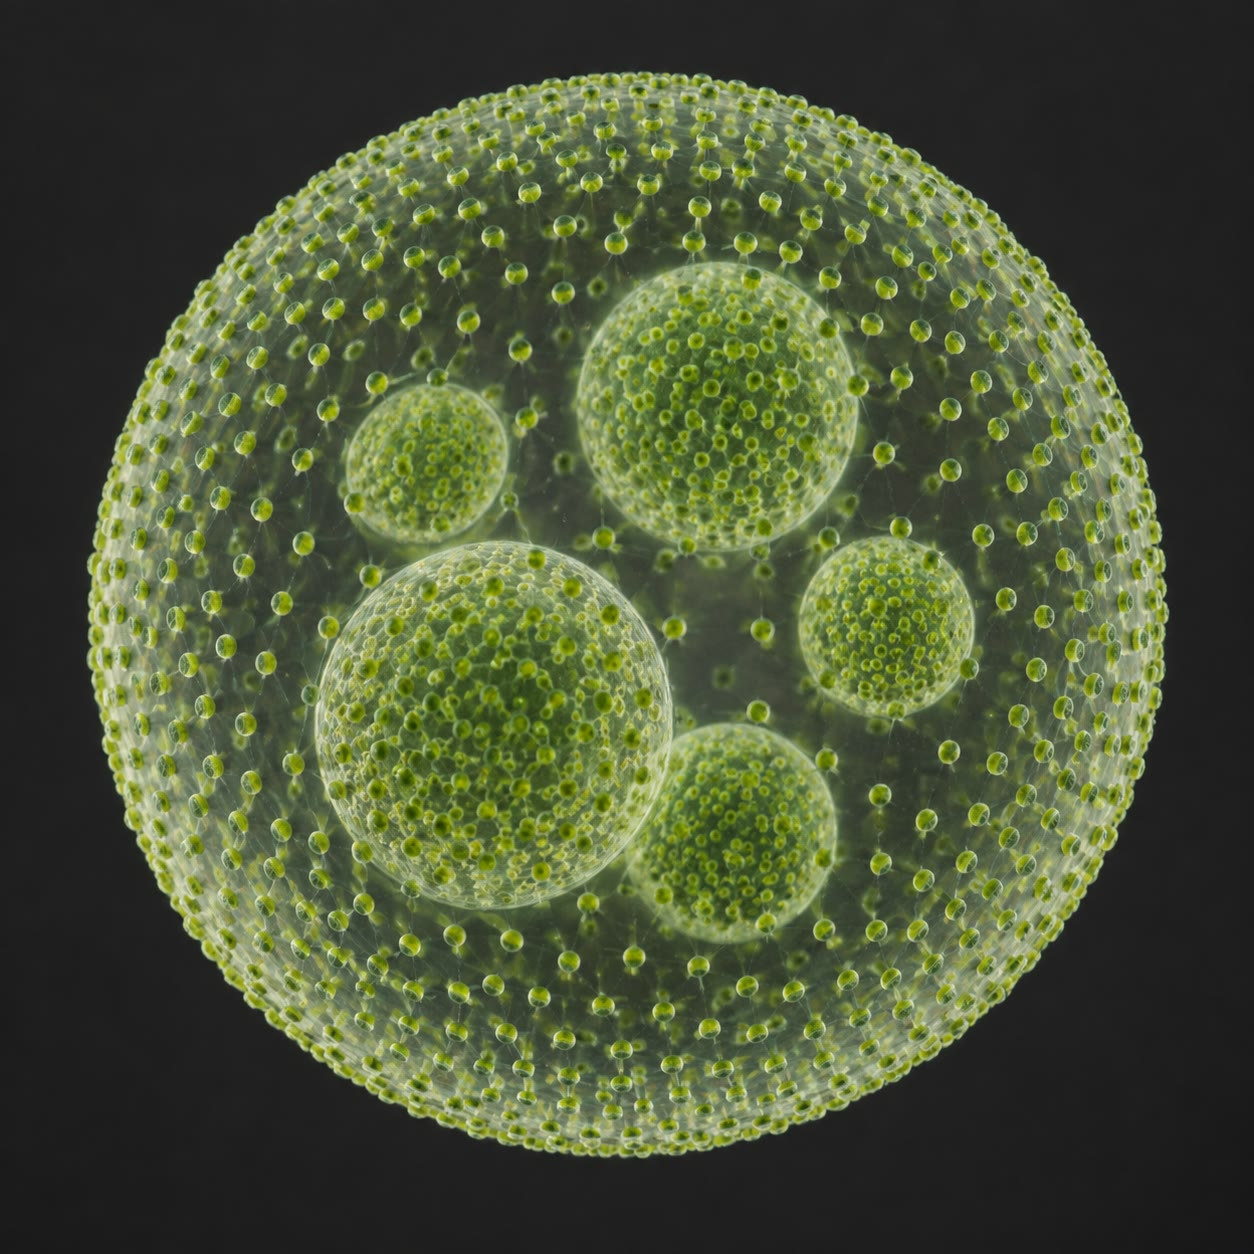
\includegraphics[width=0.55\linewidth]{images/book4/ai/b4-01-volvox.jpg}

{\small Uma colônia de \emph{Volvox}: uma esfera verde e oca de
células flageladas, com colônias-filhas crescendo em seu interior.}
\end{omfigure}

\begin{remark}[Por que dividir o trabalho?]\label{rem:b2:unicellular-diversity:whydivide}
Nessas algas, uma célula não consegue nadar e se dividir ao mesmo
tempo: os corpúsculos basais que ancoram os flagelos são necessários
para organizar o fuso. Uma célula isolada alterna; uma colônia pequena
pode se dar ao luxo de parar de nadar enquanto todas as suas células
se dividem; uma colônia grande afundaria para fora da luz (\omterm{thm:b2:unicellular-diversity:stokes}{lei de
Stokes}, \cref{thm:b2:unicellular-diversity:stokes}) durante as horas que sua divisão leva. Acima de
certo tamanho, manter algumas células nadando enquanto outras se
dividem compensa a perda dos descendentes delas --- e nasce um soma.
Os coanoflagelados, flagelados com colarinho cuja célula é uma cópia
da célula alimentar das esponjas, mostram os mesmos primeiros passos
no ramo que levou aos animais.
\end{remark}

\section{Exercícios}

\begin{exercise}[$\star$]\label{exo:b2:unicellular-diversity:1}
Defina \omterm{def:b2:unicellular-diversity:unicellular}{unicelular}, \omterm{def:b2:unicellular-diversity:unicellular}{colonial} e \omterm{def:b2:unicellular-diversity:unicellular}{multicelular}, e classifique
\emph{E.~coli}, \emph{Gonium}, \emph{Volvox} e uma célula de levedura
na categoria correta, justificando.
\end{exercise}

\begin{exercise}[$\star$]\label{exo:b2:unicellular-diversity:2}
Calcule a \omterm{prop:b2:unicellular-diversity:surface}{razão superfície/volume} de um coco de raio
\qty{0.5}{\micro m} e de um \omterm{def:b2:unicellular-diversity:protist}{protista} esférico de raio
\qty{50}{\micro m}. Qual deles respira mais depressa por unidade de
citoplasma, e por quê?
\end{exercise}

\begin{exercise}[$\star$]\label{exo:b2:unicellular-diversity:3}
Dê três diferenças estruturais entre uma bactéria e um eucarioto
\omterm{def:b2:unicellular-diversity:unicellular}{unicelular}, e uma coisa que uma ameba consegue fazer e uma bactéria
não.
\end{exercise}

\begin{exercise}[$\star$]\label{exo:b2:unicellular-diversity:4}
Indique a função de cada uma das seguintes estruturas do
\emph{Paramecium}: cílios, sulco oral, vacúolo digestivo, \omterm{prop:b2:unicellular-diversity:osmoregulation}{vacúolo
contrátil}, macronúcleo, micronúcleo.
\end{exercise}

\begin{exercise}[$\star\star$]\label{exo:b2:unicellular-diversity:5}
Com $D = \qty{5e-10}{m^2/s}$ para um metabólito no citoplasma, quanto
tempo leva a difusão através de uma bactéria de \qty{1}{\micro m} e
através de uma ameba de \qty{500}{\micro m}? Comente o que a ameba
precisa fazer e a bactéria não.
\end{exercise}

\begin{exercise}[$\star\star$]\label{exo:b2:unicellular-diversity:6}
Calcule o \omterm{prop:b2:unicellular-diversity:reynolds}{número de Reynolds} de um \emph{Paramecium} (\qty{200}{\micro
m}, \qty{1}{mm/s}), de uma bactéria (\qty{2}{\micro m}, \qty{20}{\micro
m/s}) e de um nadador humano (\qty{2}{m}, \qty{1}{m/s}), com
$\rho = \qty{1000}{kg/m^3}$ e $\eta = \qty{1e-3}{Pa.s}$. Por que um
nadador consegue deslizar após uma braçada, e uma bactéria não?
\end{exercise}

\begin{exercise}[$\star\star$]\label{exo:b2:unicellular-diversity:7}
Uma diatomácea de raio \qty{10}{\micro m} é \qty{100}{kg/m^3} mais
densa que a água. Calcule sua velocidade de sedimentação e o tempo para
cair \qty{50}{m}. Por qual fator esse tempo muda se a célula reduzir o
raio à metade? E se reduzir o excesso de densidade a
\qty{20}{kg/m^3}?
\end{exercise}

\begin{exercise}[$\star\star$]\label{exo:b2:unicellular-diversity:8}
Modele um \emph{Paramecium} como um elipsoide de semieixos \num{100},
\num{25} e \qty{25}{\micro m} ($V = \tfrac{4}{3}\pi abc$). Ele expele
o próprio volume em água a cada \qty{30}{min}. Calcule o influxo de
água em \unit{\micro m^3/s} e em litros por segundo.
\end{exercise}

\begin{exercise}[$\star\star$]\label{exo:b2:unicellular-diversity:9}
A concentração de um atraente dobra ao longo de \qty{1}{mm}. Qual é a
diferença relativa entre as duas extremidades de uma bactéria de
\qty{1}{\micro m}? E entre o início e o fim de uma corrida de
\qty{1}{s} a \qty{20}{\micro m/s}? A contagem de $N$ moléculas tem um
erro relativo de cerca de $1/\sqrt{N}$: explique por que a bactéria
compara instantes, e não lados.
\end{exercise}

\begin{exercise}[$\star\star\star$]\label{exo:b2:unicellular-diversity:10}
\emph{Thiomargarita namibiensis} é uma bactéria sulfurosa esférica de
diâmetro \qty{500}{\micro m} cujo citoplasma é uma casca de
\qty{2}{\micro m} de espessura em torno de um vacúolo de nitrato.
Calcule a razão entre sua superfície e seu volume
\emph{citoplasmático} e compare com \emph{E.~coli} (um cilindro de raio
\qty{0.5}{\micro m}; despreze as extremidades). Explique como o
vacúolo lhe permite ser tão grande, e para que serve o nitrato.
\end{exercise}

\begin{exercise}[$\star\star\star$]\label{exo:b2:unicellular-diversity:11}
Em \emph{Volvox}, as células somáticas nunca se dividem e morrem com a
colônia. Usando a restrição imposta pela flagelação e a \omterm{thm:b2:unicellular-diversity:stokes}{lei de Stokes},
explique por que essas células compensam numa colônia de \num{10000}
células, mas não numa de 16, e por que as células germinativas são as
maiores células da esfera.
\end{exercise}

\begin{exercise}[$\star\star\star$]\label{exo:b2:unicellular-diversity:12}
``\omterm{def:b2:unicellular-diversity:protist}{Protista} é um grau, não um clado.'' Explique a distinção com as
linhagens citadas neste capítulo, e diga por que a mesma afirmação é
verdadeira para ``\omterm{def:b2:unicellular-diversity:prokaryote}{procarioto}'' e falsa para ``cianobactéria''.
\end{exercise}

\section{Problema: Uma gota de água de lagoa}

\begin{problem}[{Problema de fim de semana --- uma amostra de água de
lagoa é contada, cultivada e analisada quanto à física que governa suas
células, até o balanço de água e de energia de uma alga verde}]
\label{pb:b2:unicellular-diversity:1}
Uma lagoa de \qty{1000}{m^3} é amostrada na primavera. Ao microscópio,
uma câmara de contagem cuja grade cobre \qty{1}{mm}$\times$\qty{1}{mm},
sob uma lamínula mantida \qty{0.1}{mm} acima dela, mostra 24 células
de \emph{Chlamydomonas} (esferas de raio \qty{5}{\micro m}, densidade
\qty{1050}{kg/m^3}). Considere $\rho = \qty{1000}{kg/m^3}$,
$\eta = \qty{1e-3}{Pa.s}$, $g = \qty{9.81}{m/s^2}$, $R =
\qty{8.314}{J/mol/K}$, $T = \qty{293}{K}$, $D = \qty{1.9e-9}{m^2/s}$
para o $\mathrm{CO_2}$ na água.

\medskip
\noindent\textbf{Parte I --- Contagem.}
\begin{enumerate}
  \item Calcule o volume de água sob a grade, em microlitros.
  \item Deduza a densidade de \emph{Chlamydomonas} na lagoa, em
        células por mililitro.
  \item Calcule o volume e a \omterm{prop:b2:unicellular-diversity:surface}{razão superfície/volume} de uma célula.
  \item Que fração do volume da água da lagoa é ocupada por essas
        células?
  \item Quantas \emph{Chlamydomonas} a lagoa contém?
  \item Uma cianobactéria filamentosa também está presente. Dê duas
        características visíveis ao microscópio que a distinguem da
        alga.
\end{enumerate}

\medskip
\noindent\textbf{Parte II --- Crescimento.}
A amostra é mantida na luz e contada de novo após \qty{48}{h}:
\num{384} células sob a grade.
\begin{enumerate}[resume]
  \item Calcule o \omterm{def:b2:unicellular-diversity:division}{tempo de geração} $T$.
  \item Calcule a constante de crescimento $k$ em $N = N_0 e^{kt}$, em
        \unit{h^{-1}}.
  \item Quanto tempo a população da lagoa levaria para atingir
        \qty{1e8}{} células por mililitro nesse ritmo?
  \item Dê três razões pelas quais isso não acontecerá.
  \item Se as células crescem apenas durante as \qty{12}{h} de luz do
        dia e nada à noite, quanto tempo leva o mesmo aumento?
  \item \emph{Chlamydomonas} se divide por \omterm{def:b2:unicellular-diversity:division}{fissão múltipla}, liberando
        4, 8 ou 16 filhas de uma vez. Explique por que, ainda assim, a
        contagem define bem um \omterm{def:b2:unicellular-diversity:division}{tempo de geração}.
\end{enumerate}

\medskip
\noindent\textbf{Parte III --- A física da célula.}
\begin{enumerate}[resume]
  \item Calcule o \omterm{prop:b2:unicellular-diversity:reynolds}{número de Reynolds} de uma célula que nada a
        \qty{100}{\micro m/s}.
  \item Uma célula de massa $m$ que para de bater os flagelos desliza
        por inércia uma distância $mv/(6\pi\eta r)$. Calcule-a.
  \item Calcule a velocidade de sedimentação de uma célula que parou
        de nadar.
  \item Compare o tempo para afundar \qty{1}{m} com o tempo para subir
        \qty{1}{m} nadando.
  \item A lagoa contém \qty{10}{\micro mol/L} de $\mathrm{CO_2}$
        dissolvido. Calcule o suprimento difusivo máximo de
        $\mathrm{CO_2}$ a uma célula, em moléculas por segundo.
  \item Uma célula contém \qty{100}{pg} de carbono e o duplica em uma
        geração. Calcule sua demanda média de carbono em moléculas por
        segundo, e a razão entre suprimento e demanda.
  \item Refaça a comparação para uma célula hipotética de raio
        \qty{50}{\micro m} com a mesma densidade de carbono. Conclua.
\end{enumerate}

\medskip
\noindent\textbf{Parte IV --- Água e energia.}
O citoplasma contém \qty{100}{mmol/L} de solutos; a lagoa,
\qty{1}{mmol/L}. A condutividade hidráulica da membrana é $L_p =
\qty{1e-14}{m.s^{-1}.Pa^{-1}}$ (fluxo de volume de água por unidade de
área por unidade de diferença de pressão). A hidrólise de um ATP
fornece \qty{50}{kJ/mol}; fixar um átomo de carbono custa três ATP.
\begin{enumerate}[resume]
  \item Calcule a diferença de pressão osmótica através da membrana.
  \item Calcule o volume de água que entra na célula por segundo, em
        \unit{\micro m^3/s}.
  \item Sem \omterm{prop:b2:unicellular-diversity:osmoregulation}{vacúolo contrátil}, quanto tempo a célula levaria para
        dobrar de volume?
  \item Calcule a potência mínima necessária para expulsar essa água
        contra a pressão osmótica.
  \item Converta-a em moléculas de ATP por segundo e compare com o ATP
        que a célula gasta na fixação de carbono (questão 18).
  \item Enuncie o resultado: o influxo de água da célula, o tempo que
        ela levaria para estourar e a fração de sua energia que
        manter-se sem inchar custa.
\end{enumerate}
\end{problem}
